% Fig. 2: CLEAR-Former data flow. Operations and sizes follow
% paper_build/src/deep_models.py (ApartElectricFormer) and BRIEF_REVISI.md section 3.8;
% parameter counts per path come from results/summary.json (params, components).
% Compile from this folder: pdflatex fig2_architecture.tex  ->  fig2_architecture.pdf
\documentclass[border=0.6pt]{standalone}
\usepackage[T1]{fontenc}
\usepackage{helvet}
\renewcommand{\familydefault}{\sfdefault}
\usepackage{amsmath,amssymb}
\usepackage{sansmath}
\DeclareMathSizes{6}{6}{6}{6}   % Springer: no lettering below 6 pt, sub- and superscripts included
\DeclareMathSizes{7}{7}{6}{6}
\usepackage{tikz}
\usetikzlibrary{arrows.meta,calc,fit,backgrounds,positioning}
\definecolor{ink}{HTML}{0B0B0B}
\definecolor{ink2}{HTML}{52514E}
\definecolor{edge}{HTML}{898781}
\definecolor{lane}{HTML}{F1F0EC}
\newcommand{\fs}{\fontsize{7}{8}\selectfont}
\newcommand{\fd}{\fontsize{6}{7}\selectfont}
\newcommand{\bxd}[1]{{\fd\color{ink2}#1}}
\newcommand{\by}{{\times}}
\begin{document}
\sansmath
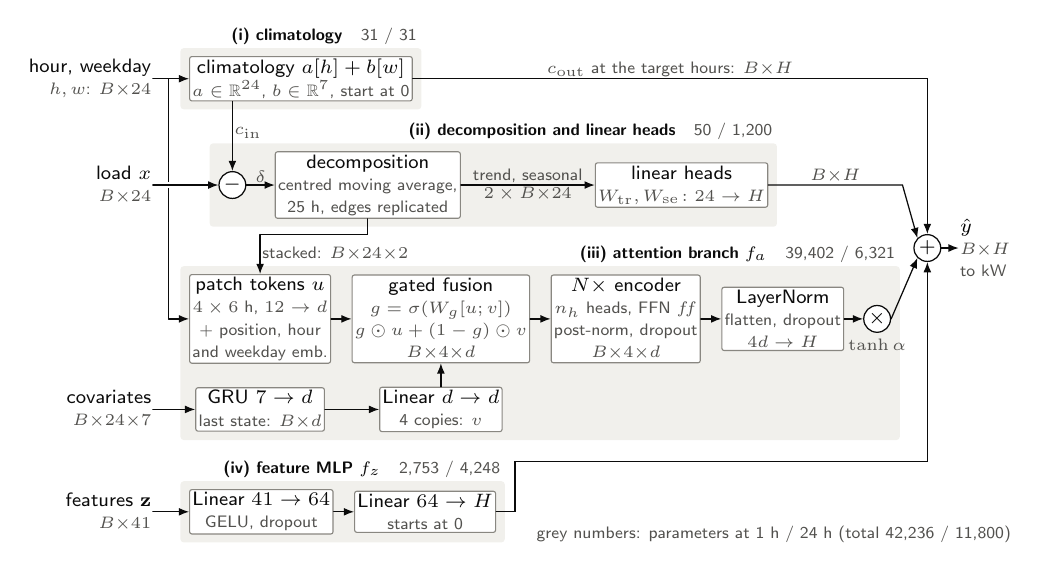
\begin{tikzpicture}[x=1mm, y=1mm, line cap=round, node distance=2.6mm,
  box/.style={draw=edge, line width=0.4pt, rounded corners=0.8pt, fill=white, align=center,
              inner xsep=1.0pt, inner ysep=1.0pt, font=\fs, text=ink},
  op/.style={circle, draw=ink, line width=0.45pt, fill=white, inner sep=0pt, minimum size=3.4mm, font=\fs},
  arr/.style={-{Latex[length=1.3mm, width=1.0mm]}, line width=0.45pt, draw=ink},
  ln/.style={line width=0.45pt, draw=ink},
  dim/.style={font=\fd, text=ink2, inner sep=0.6pt},
  inp/.style={align=right, font=\fs, text=ink, anchor=east, inner sep=0.4pt},
  ttl/.style={font=\fd\bfseries, text=ink, inner sep=0pt},
  cnt/.style={font=\fd, text=ink2, inner sep=0pt},
  pnl/.style={fill=lane, rounded corners=1.2pt, inner xsep=1.1mm, inner ysep=1.0mm},
]
% ---------------------------------------------------------------- inputs
\node[inp] (ihd)  at (16.4, 0)     {hour, weekday\\\bxd{$h, w$: $B\by24$}};
\node[inp] (ix)   at (16.4, -13.5) {load $x$\\\bxd{$B\by24$}};
\node[inp] (icov) at (16.4, -42)   {covariates\\\bxd{$B\by24\by7$}};
\node[inp] (iz)   at (16.4, -55)   {features $\mathbf{z}$\\\bxd{$B\by41$}};

% ---------------------------------------------------------------- (i) climatology
\node[box, anchor=west] (clim) at (21, 0)
  {climatology $a[h]+b[w]$\\\bxd{$a\in\mathbb{R}^{24}$, $b\in\mathbb{R}^{7}$, start at 0}};

% ---------------------------------------------------------------- (ii) decomposition and linear heads
\node[op] (minus) at (26.5, -13.5) {$-$};
\node[box, right=3.6mm of minus] (dec)
  {decomposition\\\bxd{centred moving average,}\\\bxd{25 h, edges replicated}};
\node[box, right=17mm of dec] (lin)
  {linear heads\\\bxd{$W_{\mathrm{tr}}, W_{\mathrm{se}}\colon 24\to H$}};

% ---------------------------------------------------------------- (iii) attention branch
\node[box, anchor=west] (patch) at (21, -30.5)
  {patch tokens $u$\\\bxd{$4\times 6$ h, $12\to d$}\\\bxd{+ position, hour}\\\bxd{and weekday emb.}};
\node[box, right=of patch] (gate)
  {gated fusion\\\bxd{$g=\sigma(W_g[u; v])$}\\\bxd{$g\odot u+(1-g)\odot v$}\\\bxd{$B\by4\by d$}};
\node[box, right=of gate] (enc)
  {$N\times$ encoder\\\bxd{$n_h$ heads, FFN $f\!f$}\\\bxd{post-norm, dropout}\\\bxd{$B\by4\by d$}};
\node[box, right=of enc] (head)
  {LayerNorm\\\bxd{flatten, dropout}\\\bxd{$4d\to H$}};
\node[op, right=2.4mm of head] (mult) {$\times$};
\node[dim, below=0.5mm of mult] {$\tanh\alpha$};
\node[box] (gru) at (patch |- 0,-42)
  {GRU $7\to d$\\\bxd{last state: $B\by d$}};
\node[box] (proj) at (gate |- 0,-42)
  {Linear $d\to d$\\\bxd{4 copies: $v$}};

% ---------------------------------------------------------------- (iv) feature MLP
\node[box, anchor=west] (mlp1) at (21, -55)
  {Linear $41\to 64$\\\bxd{GELU, dropout}};
\node[box, right=of mlp1] (mlp2)
  {Linear $64\to H$\\\bxd{starts at 0}};

% ---------------------------------------------------------------- sum and output
\path let \p1 = (mult.east) in node[op] (sum) at (\x1 + 4.6mm, -21.5mm) {$+$};
\node[anchor=west, align=left, font=\fs, inner sep=0.3pt] (out) at ($(sum.east)+(2.2,0)$) {$\hat{y}$\\\bxd{$B\by H$}\\\bxd{to kW}};

% ---------------------------------------------------------------- wires
\draw[ln] (18.4, 0) -- (18.4, -30.5);                                    % h, w also feed the embeddings
\draw[arr] (18.4, -30.5) -- (patch.west);
\draw[arr] (ihd.east) -- (clim.west);
\draw[white, line width=2.2pt] (17.6, -13.5) -- (19.2, -13.5);           % gap where the wires cross
\draw[arr] (ix.east) -- (minus.west);
\draw[arr] (minus.east) -- node[dim, above] {$\delta$} (dec.west);
\draw[arr] (minus.north |- clim.south) -- (minus.north) node[dim, pos=0.45, right] {$c_{\mathrm{in}}$};
\draw[arr] (dec.east) -- node[dim, above] {trend, seasonal} node[dim, below] {$2\times B\by24$} (lin.west);
\coordinate (br) at ($(dec.south)+(0,-2.0)$);
\draw[ln] (dec.south) -- (br) -- (patch.north |- br);
\draw[arr] (patch.north |- br) -- (patch.north) node[dim, pos=0.5, right] {stacked: $B\by24\by2$};
\draw[arr] (patch.east) -- (gate.west);
\draw[arr] (gate.east) -- (enc.west);
\draw[arr] (enc.east) -- (head.west);
\draw[arr] (head.east) -- (mult.west);
\draw[arr] (icov.east) -- (gru.west);
\draw[arr] (gru.east) -- (proj.west);
\draw[arr] (proj.north) -- (gate.south);
\draw[arr] (iz.east) -- (mlp1.west);
\draw[arr] (mlp1.east) -- (mlp2.west);
\draw[arr] (clim.east) -- node[dim, above, pos=0.5] {$c_{\mathrm{out}}$ at the target hours: $B\by H$} (sum.north |- clim.east) -- (sum.north);
\coordinate (lj) at ($(sum.north west)+(-1.9,0)$);
\draw[arr] (lin.east) -- node[dim, above, pos=0.5] {$B\by H$} (lj |- lin.east) -- (sum.north west);
\draw[arr] (mult.east) -- (sum.south west);
\coordinate (fz) at ($(mlp2.east)+(2.4,0)$);
\draw[arr] (mlp2.east) -- (fz) -- (fz |- 0,-48.6) -- (sum.south |- 0,-48.6) -- (sum.south);
\draw[arr] (sum.east) -- (out.west);

% ---------------------------------------------------------------- path panels and titles
\begin{scope}[on background layer]
  \node[pnl, fit=(clim)] (p1) {};
  \node[pnl, fit=(minus) (dec) (lin)] (p2) {};
  \node[pnl, fit=(patch) (gate) (enc) (head) (mult) (gru) (proj)] (p3) {};
  \node[pnl, fit=(mlp1) (mlp2)] (p4) {};
\end{scope}
\node[ttl, anchor=south east] at ($(p1.north east)+(-0.6,0.35)$) {(i) climatology\quad\textmd{\color{ink2}31 / 31}};
\node[ttl, anchor=south east] at ($(p2.north east)+(-0.6,0.35)$) {(ii) decomposition and linear heads\quad\textmd{\color{ink2}50 / 1,200}};
\node[ttl, anchor=south east] at ($(p3.north east)+(-0.6,0.35)$) {(iii) attention branch $f_a$\quad\textmd{\color{ink2}39,402 / 6,321}};
\node[ttl, anchor=south east] at ($(p4.north east)+(-0.6,0.35)$) {(iv) feature MLP $f_z$\quad\textmd{\color{ink2}2,753 / 4,248}};
\node[cnt, anchor=south east] at (out.east |- p4.south) {grey numbers: parameters at 1 h / 24 h (total 42,236 / 11,800)};
\end{tikzpicture}
\end{document}
